\hypertarget{basic-settings}{%
\subsection{Basic Settings}\label{basic-settings}}

Here we present the basic setup of the model.

\hypertarget{coordinate-system}{%
\subsubsection{Coordinate System}\label{coordinate-system}}

The coordinate system of the atmospheric model consists of longitude \(\lambda\), latitude
\(\varphi\), and normalized pressure \(\eta\) (definitions are given
below), each of which is treated as orthogonal.
However, \(z\) is used
for the vertical coordinate in the ground, which is treated in a land physics component.

Longitude is discretized at equal intervals
(\texttt{SUBROUTINE:\ {[}SETLO{]}} in asetc.F).
\begin{eqnarray}
  \lambda_i = 2 \pi \frac{i-1}{I},  \;\;\; i = 1, \ldots I.
\end{eqnarray}

Latitude grids \(\varphi_j\) are derived from the
Gauss-Legendre integral formula (\texttt{SUBROUTINE:\ {[}SETLA{]}} in
asetc.F).
This is the zero point of the Legendre polynomial of order J
with \(\mu = \sin \varphi\) as the argument
(\texttt{SUBROUTINE:\ {[}GAUSS{]}} in uspst.F).
If J is large, we can approximate
\begin{eqnarray}
  \varphi_j =  \pi \left( \frac{1}{2}- \frac{j-1/2}{J} \right), \;\;\; j = 1, \ldots J.
\end{eqnarray}
Usually, the grid spacing of longitude and latitude is taken to be
approximately equal to \(J = I/2\), based on the triangular truncation of the spectral method.

Air pressure \(p\) is defined at half levels
(\(p_{k+1/2},\ k = 1, 2, \ldots K\)) using the following formula using
constants \(A_{k+1/2},\ B_{k+1/2}\):
\begin{eqnarray}
p_{k+1/2} = A_{k+1/2} +B_{k+1/2}\,p_s,
\end{eqnarray}
where \(A_{1/2}=A_{K+1/2}=0,\ B_{1/2}=1,\ B_{K+1/2}=0\) and thus
\(p_{1/2}=p_s,\ p_{K+1/2}=0\).
Therefore, the normalized pressure
\(\sigma\equiv p/p_s\) can be written as below:
\begin{eqnarray}
\sigma_{k+1/2} = \frac{A_{k+1/2}}{p_s} +B_{k+1/2}.
\end{eqnarray}

Furthermore, a hybrid normalized pressure \(\eta\) is defined as below:
\begin{eqnarray}
\eta_{k+1/2} = \frac{A_{k+1/2}}{p_0} +B_{k+1/2},\ \ \ p_0\equiv 1000\ \mathrm{hPa}.
\end{eqnarray}

Since \(A_{k+1/2},\ B_{k+1/2}, p_0\) are constants, \(\eta_{k+1/2}\) is
also a constant and we use it as the vertical coordinate of the
atmopheric model.
However, as described in Chapter 2, basic equations
are descretized in such a way that \(\eta_{k+1/2}\) does not explicitly
appear and \(\sigma_{k+1/2}\) is used instead to commonize source codes
with the \(\sigma\)-coordinate system used in MIROC 5.

Air pressure \(p_k\) at full levels (\(p_k,\ k=1,2,\ldots K)\) is
interpolated from half-level pressure as below:
\begin{eqnarray}
 p_k = \left\{ \frac{1}{1+\kappa}
                     \left( \frac{  p^{\kappa +1}_{k-1/2}
                                  - p^{\kappa +1}_{k+1/2}      }
                                  { p_{k-1/2} - p_{k+1/2} }
                     \right)
              \right\}^{1/\kappa}.
\end{eqnarray}
Full-level pressure in a 80-level configuration is shown in Fig.
\ref{levels}. While lower layers follow the terrain, upper layers are
isobaric, and the two are smoothly connected.

\begin{figure}
\centering
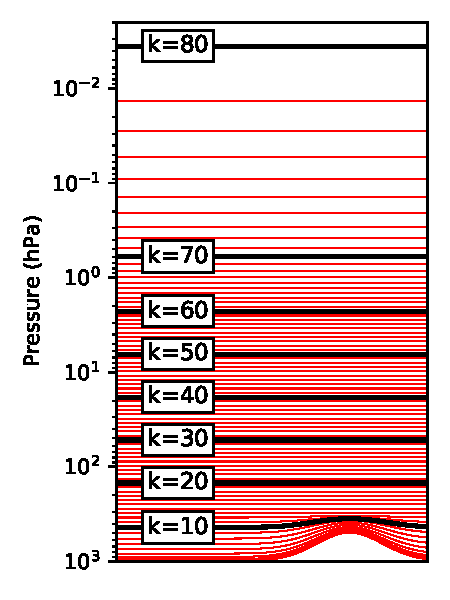
\includegraphics{levels.pdf}
\caption{Default arangement of vertical levels for 80-level
simulation.\label{levels}}
\end{figure}

All prognostic variables are defined either on a grid of
\((\lambda_i, \varphi_j, \eta_k)\) or \((\lambda_i, \varphi_j, z_l)\).
(The underground level, \(z_l\), is described in the section on physical
processes.)

In the time direction, the forecast equations are discretized at
evenly spaced \(\Delta t\) and time integration is performed.
However, \(\Delta t\) may change in cases where the stability of the time integration is insufficient.

\hypertarget{physical-constants}{%
\subsubsection{Physical Constants}\label{physical-constants}}

The basic physical constants are shown below
(\texttt{SUBROUTINE\ {[}PCONST{]}} in apcon.F).

\setlength\LTleft{0pt}\setlength\LTright{0pt}
\begin{longtable}[]{@{}llll@{}}
\toprule\relax
Element & Symbol & Unit & Value\tabularnewline
\midrule\relax
\endhead
Earth radius & \(a\) & m & 6.37 \(\times 10^6\)\tabularnewline
Gravitational acceleration & \(g\) & m s\(^{-2}\) & 9.8\tabularnewline
Atmospheric specific heat at constant pressure & \(C_p\) & J kg\(^{-1}\)
K\(^{-1}\) & 1004.6\tabularnewline
Atmospheric gas constant & \(R\) & J kg\(^{-1}\) K\(^{-1}\) &
287.04\tabularnewline
Latent heat of water evaporation & \(L\) & J kg\(^{-1}\) & 2.5
\(\times 10^6\)\tabularnewline
Water vapor specific heat at constant pressure & \(C_v\) & J kg\(^{-1}\)
K\(^{-1}\) & 1810\tabularnewline
Gas constant of water & \(R_v\) & J kg\(^{-1}\) K\(^{-1}\) &
461\tabularnewline
Density of liquid water & \(d_{H_2O}\) & kg m\(^{-3}\) &
1000\tabularnewline
Saturated vapor pressure at 0 \(^{\circ}\)C & \(e^*\)(273K) & Pa &
611\tabularnewline
Stefan-Bolzman constant & \(\sigma_{SB}\) & W m\(^{-2}\) K\(^{-4}\) &
5.67 \(\times 10^{-8}\)\tabularnewline
Kárman constant & \(k\) & & 0.4\tabularnewline
Latent heat of ice melting & \(L_M\) & J kg\(^{-1}\) & 3.4
\(\times 10^5\)\tabularnewline
Freezing point of water & \(T_M\) & K & 273.15\tabularnewline
Constant pressure specific heat of water & \(C_w\) & J kg\(^{-1}\) &
4200\tabularnewline
Freezing point of seawater & \(T_I\) & K & 271.35\tabularnewline
Specific heat ratio of ice at constant pressure &
\(C_I = C_w - L_M/T_M\) & & 2397\tabularnewline
Water vapor molecular weight ratio & \(\epsilon = R/R_v\) & &
0.622\tabularnewline
Coefficient of virtual temperature & \(\epsilon_v = \epsilon^{-1} - 1\)
& & 0.606\tabularnewline
Ratio of specific heat to gas constant & \(\kappa = R/C_p\) & &
0.286\tabularnewline
\bottomrule
\end{longtable}
